\section{Risultati ottenuti}
\subsection{Metriche utilizzate per detection su singole immagini}
Nell'ambito della computer vision vengono tipicamente utilizzate due tipi di metriche per misurare due diverse proprietà:
\begin{itemize}
\item Corretta determinazione della posizione degli oggetti;
\item Rilevamento dell'esistenza degli oggetti nell'immagine e la loro corretta classificazione.
\end{itemize}
Le metriche utilizzate per misurare la bontà dei risultati del progetto sono F1, AP (Average Precision) e mAp (mean Average Precision) le quali misurano la seconda proprietà sopra elencata.
Prima di iniziare a descrivere le metriche è necessario definire alcuni concetti che saranno poi coinvolti per il calcolo dei valori delle metriche.
\subsubsection{Precision}
La precision misura l'accuratezza delle classificazioni ed indica la percentuale di classificazioni corrette sulla base di quelle totali e viene calcolata come:
\[
    precision = \frac{TP}{TP + FP}
\]
Dove TP (True Positives) è il numero di classificazioni corrette e FP (False Positives) è il numero di classificazioni errate. E' da sottolineare che se uno stesso elemento viene individuato più di una volta, solo la prima volta conterà come TP mentre il resto delle volte conterà come FP. Questa metrica fornisce un'idea sulla correttezza dei risultati.
\subsubsection{Recall}
La recall misura quanti oggetti sono stati individuati e classificati correttamente sulla base degli oggetti totali, viene calcolata come:
\[
    recall = \frac{TP}{TP + FN}
\]
Dove TP (True Positives) è sempre il numero di classificazioni corrette mentre FN (False Negatives) è il numero di di oggetti che non sono stati individuati ma che se sarebbe stato corretto individuare. Questa metrica fornisce un'idea sulla completezza dei risultati.
\subsubsection{F1}
F1 è una metrica che combina la precision con il recall e può essere interpretata come la media armonica tra la precision e la recall. Il valore massimo ottenibile è 1 raggiungibile nel caso in cui sia la precision che la recall siano pari ad 1 mentre il valore minimo è 0 ottenuto quando entrambe le metriche che lo compongono assumono valore pari a 0. Viene calcolato come:
\[
    F1 = 2 \times \frac{precision \times recall}{precision + recall}
\]
\subsubsection{Intersection over union}
L'intersection over union (IoU) misura il grado di sovrapposizione tra due aree e viene usato per misurare il grado di sovrapposizione tra la box dell'oggetto individuato e la box dell'oggetto reale. Viene calcolata come:
\[
    IoU = \frac{AI}{AU}
\]
Dove AI (Area dell'Intersezione) corrisponde all'area dell'intersezione tra le due bounding boxes e AU (Area dell'Unione) corrisponde all'area dell'unione tra le due bounding boxes.
Una label per essere considerata come corretta deve avere un valore di IoU maggiore di una soglia stabilità (per esempio 0.5).
\begin{figure}[H]
	\centering
	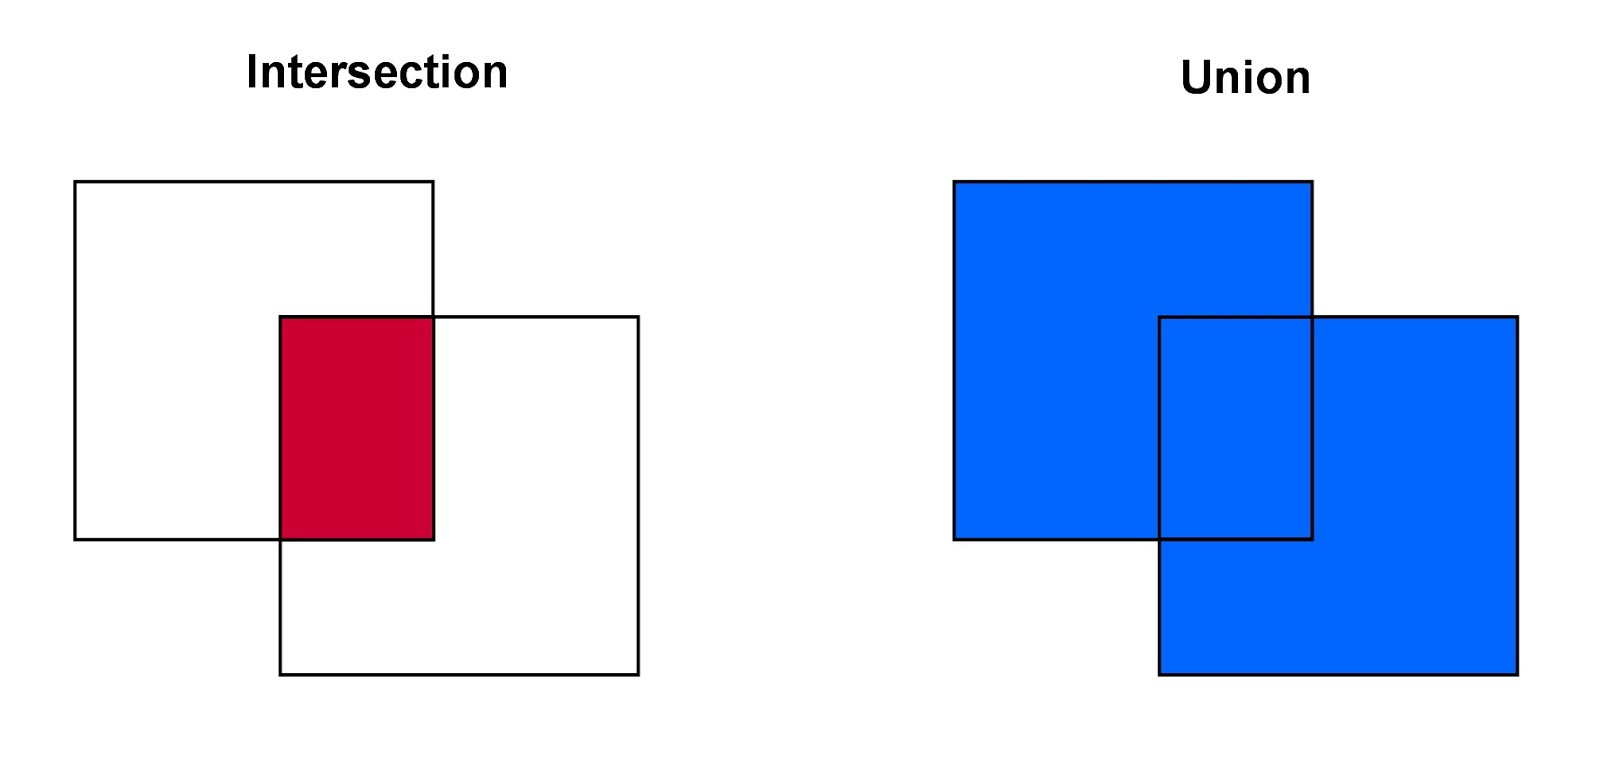
\includegraphics[width=0.5\linewidth]{images/unione-intersezione.jpg}
	\caption{Esempio di intersezione e di unione}
	\label{Esempio di intersezione e di unione}
\end{figure}
\subsubsection{Average Precision}
Un'altra delle metriche utilizzate è l'average precision (AP) e per calcolarla si fa la media delle precisioni di undici diversi valori di recall equamente distribuiti. Questa metrica viene applicata ad una sola categoria di elementi e viene calcolata tramite la seguente formula:
\[
    AP = \frac{1}{11}\sum_{Recall\ped{i}}^{} Precision(Recall\ped{i})
\]
Dove \textit{i}=[0, 0.1, 0.2, …, 1.0] in quanto 0 \textless =recall\textless =1. Inoltre la precisione di uno specifico valore di recall viene calcolata nel seguente modo:
\[
    Precision(Recall\ped{i}) = max\,Precision(Recall\ped{j}) \quad \textrm{and} \quad j>=i
\]
L'AP è un valore che riassume la forma della curva precision/recall per una data categoria.
\subsubsection{Mean Average Precision}
La mean average precision (mAP) è la media delle AP di tutte le categorie calcolata su diverse soglie di IoU:
\[
    mAP\ped{IoU=x\%} = \frac{1}{n}\sum_{i=0}^{n}AP\ped{i}
\]
Dove \textit{i} è il numero totale di categorie sulle quali è stata calcolata la propria AP e \textit{x} rappresenta diverse soglie di IoU.

\subsection{Dataset utilizzato per detection su singole immagini}
I test sono stati eseguiti su un dataset di immagini satellitari in alta risoluzione con circa 3000 pixels di altezza e 4000 di larghezza. Il modello di rete è stato allenato per riconoscere elementi appartenenti a sessanta categorie, le quali, verranno riportate nella tabella 1 insieme ai loro relativi risultati. Il dataset utilizzato è particolarmente impegnativo da analizzare a causa delle ambiguità tra molte delle sue categorie in quanto molte di esse rappresentano lo stesso elemento ma sotto forma di tipologie diverse. Per esempio, gli oggetti appartenenti alle categorie dalla 8 alla 17 sono tutti dei camion, ma di diversa tipologia, tanto che perfino un essere umano, se non esperto in materia, farebbe fatica a distinguerli. La seconda difficoltà viene aggiunta dal fatto che le immagini sono state prese da satelliti i quali orbitano ad un'altezza di migliaia di kilometri dalla superficie terrestre. Data l'enorme distanza, gli oggetti di dimensioni minori come le automobili sono molto difficili da individuare ed ancora più complesso lo è classificarli nella loro corretta categoria. E' per questo motivo che viene applicata la frammentazione visto che risulta fondamentale non perdere risoluzione durante la detection. In seguito, svolge un ruolo fondamentale l'algoritmo di ricostruzione dell'immagine frammentata in quanto permette di ricomporre le bounding boxes di quegli elementi che sono stati suddivisi su più regioni. In seguito viene mostrata una delle immagini presa dal dataset utilizzato per calcolare le metriche.
\begin{figure}[H]
	\centering
	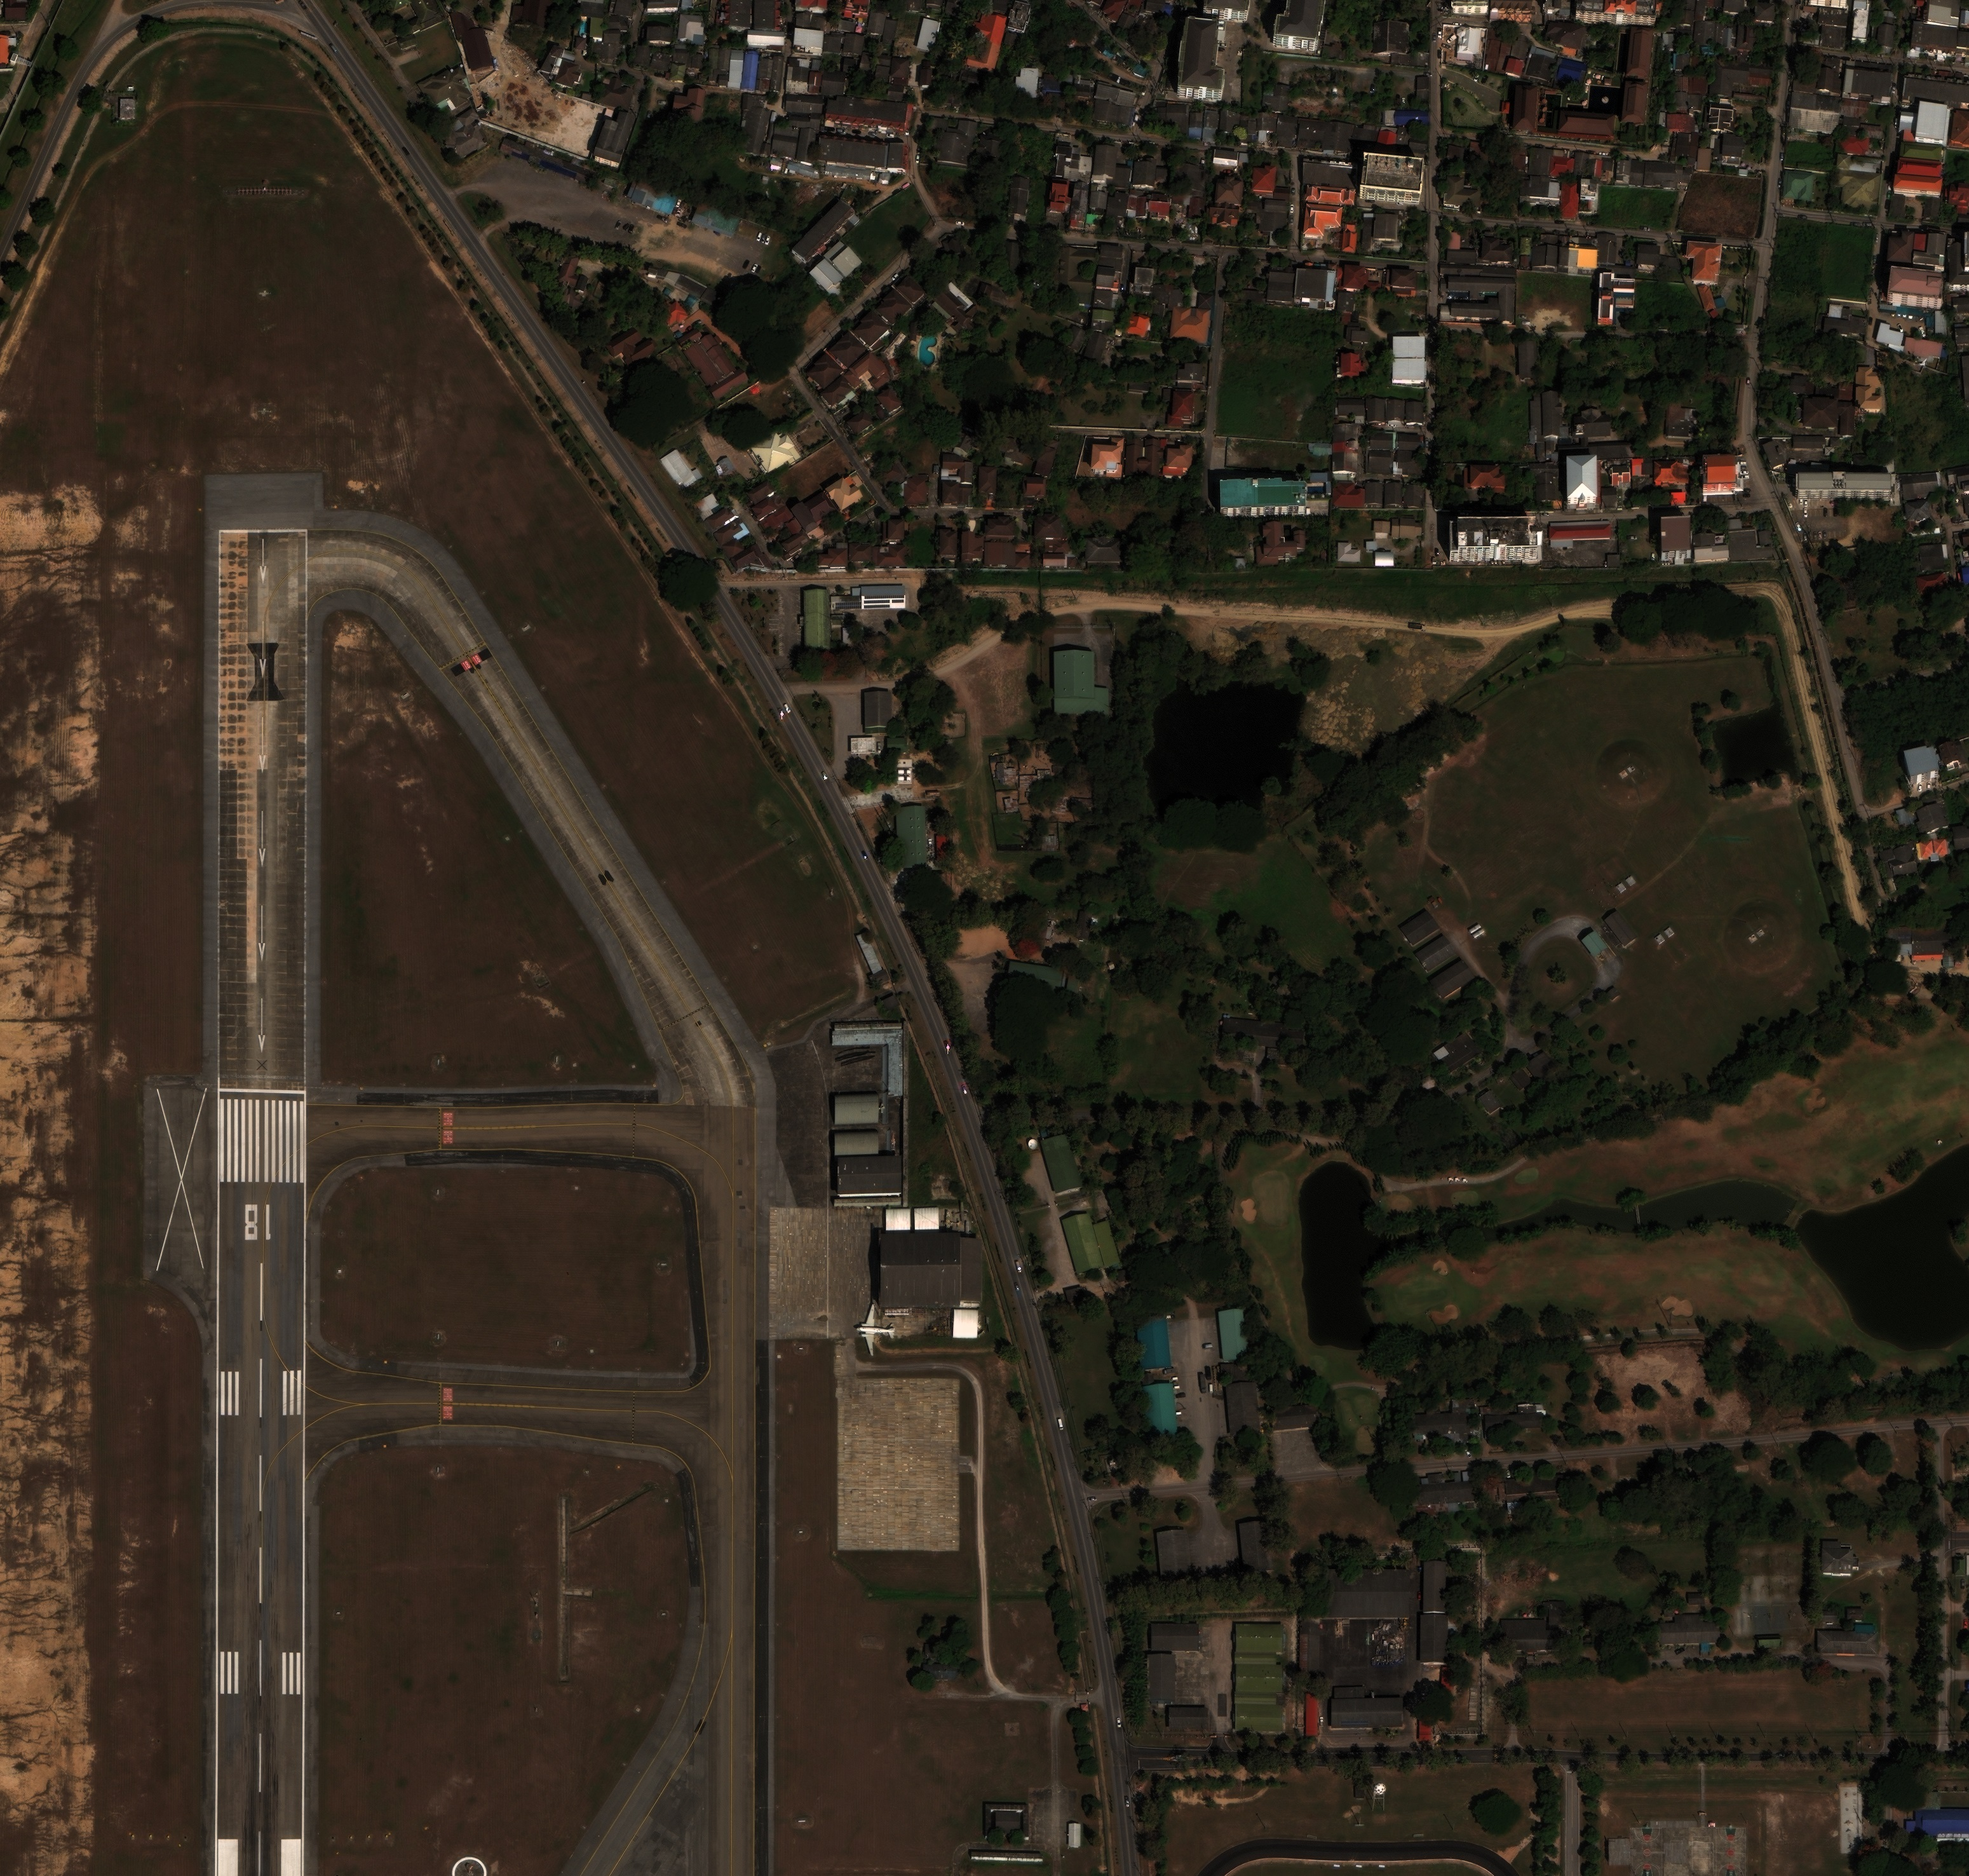
\includegraphics[width=0.7\linewidth]{images/immagine-satellite.jpg}
	\caption{Immagine satellitare appartenente al dataset utilizzato}
	\label{Immagine satellitare appartenente al dataset utilizzato}
\end{figure}

\subsubsection{Impostazione parametri detection}
Il parametro utilizzato per determinare quali labels tenere tra tutte quelle risultanti da una detection è
l' \textbf{affidabilità}.\\
Nella seguente listea vengono elencati i parametri che intervengono in fase di ricostruzione delle labels a seguito della detection:
\begin{itemize}
\item \textbf{Dimensione regioni};
\item \textbf{Dimensione stride};
\item \textbf{Overlap};
\item \textbf{Tolleranza};
\item \textbf{Soglia di matching}.
\end{itemize}
Una spiegazione più dettagliata riguardo ai parametri la si può trovare in sezione \textit{4.1} o nel \textit{Glossario}.
Ogni immagine è stata suddivisa in regioni da 640x640 pixels. A causa della difficoltà nell'individuazione degli elementi, il loro score sarà relativamente basso risultando quindi in una scarsa affidabilità. La \textbf{soglia di affidabilità} per la \textbf{condizione di correlazione} necessaria per effettuare un match è stata perciò impostata a 0. Di conseguenza, due labels di diversa categoria non potranno mai venire unite. Le altre funzioni ridefinibili sono state lasciate con il loro comportamento di default descritto in sezione \textit{4.1}. I restanti parametri sono invece variabili e ne sono state testate diverse combinazioni ai fini di ricercare quelle combinazioni di parametri in grado di fornire i risultati migliori.
\\
In totale sono state testate 4 soglie diverse di \textbf{affidabilità}=[0.01, 0.1, 0.2, 0.3], 3 valori di \textbf{overlap}=[0, 1, 2], 3 di \textbf{tolleranza}=[0, 1, 2], 4 \textbf{soglie di matching}=[20\%, 40\%, 60\%, 80\%] per un totale di 144 combinazioni di parametri diverse. Le metriche sono state calcolate come media delle metriche per ogni combinazione di parametri e per ogni singola immagine.\\
Per quanto riguarda il test, una bounding box individuata tramite detection è considerata come corretta solo se la sua IoU con la bounding box reale è maggiore di una certa soglia di Iou. Questa soglia è la stessa soglia utilizzata per il calcolo di dell'mAP. Per effettuare i test questa soglia è stata fissata al 50\%.

\subsection{Risultati ottenuti nella detection su singole immagini}
Nella seguente sezione vengono riportati i risultati ottenuti per misurare la qualità della detection e della frammentazione.
\subsubsection{Risultati per categoria}
Nella tabella sottostante vengono riportate tutte le 60 categorie coinvolte nel test insieme al loro AP. I valori mostrati sono quelli relativi alla migliore combinazione di parametri per ogni specifica categoria. La detection è stata effettuata con \textbf{affidabilità} 0.01 in quanto questo è il valore che massimizza i valori di AP e mAP. AP (Original) mostra il valore dell'AP dopo avere effettuato la detection con frammentazione, AP (NMS) è il valore dell'AP dopo aver applicato NMS ed infine AP è il valore dell'AP calcolato dopo aver applicato l'algoritmo di ricostruzione dell'immagine frammentata.

\newpage
\begin{center}
\begin{longtable}{|c|l|c|c|c|}

\hline \multicolumn{1}{|c|}{\textbf{Numero}} &
\multicolumn{1}{c|}{\textbf{Categoria}} & \multicolumn{1}{c|}{\textbf{AP (Original)}} &\multicolumn{1}{c|}{\textbf{AP (NMS)}} &\multicolumn{1}{c|}{\textbf{AP}} \\ \hline\endfirsthead

\hline \multicolumn{1}{|c|}{\textbf{Numero}} &
\multicolumn{1}{c|}{\textbf{Categoria}} &\multicolumn{1}{c|}{\textbf{AP (Original)}} &\multicolumn{1}{c|}{\textbf{AP (NMS)}} &\multicolumn{1}{c|}{\textbf{AP}}\\ \hline \endhead

\hline \multicolumn{5}{|c|}{{------ Continua nella pagina successiva ------}} \\ \hline
\endfoot

\hline

\caption{Lista delle categorie del dataset utilizzato per effettuare i test con relativo AP}
\label{lista categorie} \\

\endlastfoot


1 & Fixed-wing Aircraft & 0.224319 & 0.225709 & 0.234913\\
2 & Small Aircraft & 0.423006 & 0.421561 & 0.487984\\
3 & Cargo Plane & 0.793246 & 0.780495 & 0.809706\\
4 & Helicopter & 0.343750 & 0.343750 & 0.455165\\
5 & Passenger Vehicle & 0.000514 & 0.000561 & 0.000616\\
6 & Small Car & 0.360364 & 0.349376 & 0.354816\\
7 & Bus & 0.320155 & 0.319980 & 0.322155\\
8 & Pickup Truck & 0.004013 & 0.003817 & 0.003832\\
9 & Utility Truck & 0.022319 & 0.022180 & 0.022249\\
10 & Truck & 0.093073 & 0.096008 & 0.097272\\
11 & Cargo Truck & 0.112346 & 0.110611 & 0.113069\\
12 & Truck w/Box & 0.405223 & 0.382302 & 0.389924\\
13 & Truck Tractor & 0.011702 & 0.011205 & 0.011360\\
14 & Trailer & 0.128112 & 0.118257 & 0.121111\\
15 & Truck w/Flatbed & 0.083729 & 0.084326 & 0.086383\\
16 & Truck w/Liquid & 0.028560 & 0.029433 & 0.029457\\
17 & Crane Truck & 0.070424 & 0.070487 & 0.103344\\
18 & Railway Vehicle & 0.00000 & 0.00000 & 0.00000\\
19 & Passenger Car & 0.621967 & 0.634951 & 0.653586\\
20 & Cargo Car & 0.528376 & 0.535936 & 0.537790\\
21 & Flat Car & 0.408165 & 0.436869 & 0.436869\\
22 & Tank Car & 0.000501 & 0.000552 & 0.000563\\
23 & Locomotive & 0.492844 & 0.498693 & 0.500454\\
24 & Maritime Vessel & 0.132787 & 0.122395 & 0.137974\\
25 & Motorboat & 0.304536 & 0.309246 & 0.317420\\
26 & Sailboat & 0.476163 & 0.492080 & 0.501056\\
27 & Tugboat & 0.375028 & 0.379075 & 0.385908\\
28 & Barge & 0.229450 & 0.232367 & 0.237915\\
29 & Fishing Vessel & 0.131085 & 0.134347 & 0.145607\\
30 & Ferry & 0.451626 & 0.445131 & 0.494575\\
31 & Yacht & 0.554554 & 0.561531 & 0.583826\\
32 & Container Ship & 0.562968 & 0.555579 & 0.624139\\
33 & Oil Tanker & 0.562263 & 0.615124 & 0.615124\\
34 & Engineering Vehicle & 0.114510 & 0.114657 & 0.116365\\
35 & Tower Crane & 0.012496 & 0.007083 & 0.007517\\
36 & Container Crane & 0.053083 & 0.050028 & 0.060336\\
37 & Reach Stacker & 0.314528 & 0.317667 & 0.320265\\
38 & Straddle Carrier & 0.573863 & 0.572912 & 0.574765\\
39 & Mobile Crane & 0.131302 & 0.139258 & 0.155806\\
40 & Dump Truck & 0.166618 & 0.169499 & 0.169579\\
41 & Haul Truck & 0.868698 & 0.859369 & 0.889144\\
42 & Scraper/Tractor & 0.028915 & 0.028613 & 0.031487\\
43 & Front Loader/Bulldozer & 0.129784 & 0.138587 & 0.140348\\
44 & Excavator & 0.340663 & 0.335421 & 0.336678\\
45 & Cement Mixer & 0.173915 & 0.182477 & 0.182591\\
46 & Ground Grader & 0.266859 & 0.265571 & 0.265616\\
47 & Hut/Tent & 0.025208 & 0.023967 & 0.026293\\
48 & Shed & 0.009840 & 0.009854 & 0.010107\\
49 & Building & 0.535869 & 0.482216 & 0.490359\\
50 & Aircraft Hangar & 0.019961 & 0.025452 & 0.027149\\
51 & Damaged Building & 0.020142 & 0.021223 & 0.022819\\
52 & Facility & 0.125133 & 0.114053 & 0.139637\\
53 & Construction Site & 0.017198 & 0.016450 & 0.016892\\
54 & Vehicle Lot & 0.087038 & 0.081471 & 0.095994\\
55 & Helipad & 0.020963 & 0.022512 & 0.022866\\
56 & Storage Tank & 0.453776 & 0.452578 & 0.474606\\
57 & Shipping Container Lot & 0.159574 & 0.140996 & 0.149238\\
58 & Shipping Container & 0.101220 & 0.102641 & 0.102708\\
59 & Pylon & 0.657612 & 0.661616 & 0.661769\\
60 & Tower & 0.070426 & 0.071527 & 0.071872\\
\end{longtable}
\end{center}

Osservando i risultati si può subito notare che per ogni categoria si ha che AP$>=$AP(NMS) notando quindi un miglioramento delle metriche a seguito dell'applicazione dell'algoritmo. Per alcune categorie si ha che AP$=$AP(NMS), in questi casi significa che nessuna delle bounding boxes relative a quella categoria è stata coinvolta nella frammentazione. Per alcune categorie può succedere che AP(Original) risulti maggiore sia di AP(NMS) che di AP, questo fenomeno si verifica con più frequenza in presenza di molti oggetti parzialmente sovrapposti tra loro. In questo caso NMS potrebbe causare delle imprecisioni scartando delle bounding boxes che dovrebbero essere in realtà mantenute. Alcune categorie come la numero 5 e la numero 8 presentano un valore di AP particolarmente basso. Si tratta di oggetti che a causa della bassa risoluzione risultano molto piccoli ed ambigui perfino per un occhio umano, per cui, anche il modello spesso commette errori nella loro individuazione e classificazione.
\begin{figure}
\begin{center}
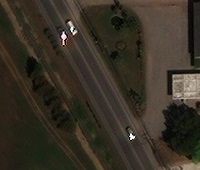
\includegraphics[width=0.4\textwidth, height=0.25\textheight]{images/auto1-satellite.jpg}
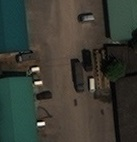
\includegraphics[width=0.4\textwidth, height=0.25\textheight]{images/auto2-satellite.jpg}
\end{center}
\caption{Esempi di oggetti molto difficili da individuare e classificare}
\end{figure}

\clearpage
\subsubsection{Risultati per parametri}
La seguente tabella mostra riporta i risultati ottenuti con diverse combinazioni di parametri mostrando i valori di F1 e mAP. mAP(NMS) indica il valore dell'mAp calcolato dopo aver effettuato NMS sull'immagine frammentata mentre mAP è il valore dell'mAP calcolato dopo aver applicato l'algoritmo di ricostruzione dell'immagine frammentata riportandone anche l'aumento in percentuale.

\begin{table}[h!]
\centering
\begin{tabular}{|c|c|c|c|c|c|c|} 
\hline
Stride & Overlap & Tolleranza & Match & F1 & mAP(NMS) & mAP\\ [0.5ex] 
\hline
0 & 0 & 0 & 0 & 0 & 0 & 0 (+0.0\%)\\
0 & 0 & 0 & 0 & 0 & 0 & 0 (+0.0\%)\\
0 & 0 & 0 & 0 & 0 & 0 & 0 (+0.0\%)\\
0 & 0 & 0 & 0 & 0 & 0 & 0 (+0.0\%)\\
0 & 0 & 0 & 0 & 0 & 0 & 0 (+0.0\%)\\
0 & 0 & 0 & 0 & 0 & 0 & 0 (+0.0\%)\\
0 & 0 & 0 & 0 & 0 & 0 & 0 (+0.0\%)\\
0 & 0 & 0 & 0 & 0 & 0 & 0 (+0.0\%)\\
0 & 0 & 0 & 0 & 0 & 0 & 0 (+0.0\%)\\
0 & 0 & 0 & 0 & 0 & 0 & 0 (+0.0\%)\\
0 & 0 & 0 & 0 & 0 & 0 & 0 (+0.0\%)\\
0 & 0 & 0 & 0 & 0 & 0 & 0 (+0.0\%)\\
0 & 0 & 0 & 0 & 0 & 0 & 0 (+0.0\%)\\
0 & 0 & 0 & 0 & 0 & 0 & 0 (+0.0\%)\\
0 & 0 & 0 & 0 & 0 & 0 & 0 (+0.0\%)\\
0 & 0 & 0 & 0 & 0 & 0 & 0 (+0.0\%)\\
\hline
\end{tabular}
\caption{Risultati generali detection con diversi parametri}
\label{lista risultati}
\end{table}

\subsection{Metriche utilizzate per tracking su video}
L'obiettivo del tracking è quello di identificare tutti gli oggetti in un video e tracciarli nel tempo. Quest'ultimo compito viene svolto assegnando un ID unico a ciascun oggetto assicurandosi che esso rimanga lo stesso per tutta la durata del video. Di conseguenza nel tracking sono due gli aspetti fondamentali di cui tenere conto:
\begin{itemize}
\item Precisione con cui viene determinata la locazione di un oggetto;
\item Correttezza del tracciamento (anche in presenza di occultamento, perdita di qualità, etc...)
\end{itemize}
In seguito vengono descritte le metriche utilizzare per valutare la qualità del tracciamento.

\subsubsection{Mostly Tracked Trajectories}
Mostly Tracked Trajectories (MT), misura la percentuale di elementi, rispetto a quelli totali, che sono stati tracciati correttamente per almeno l'80\% della loro traiettoria. Indica quindi la correttezza del tracciamento, valori più alti sono considerati migliori.
\subsubsection{Mostly Lost Trajectories}
Mostly Lost Trajectories (ML), misura la percentuale di elementi, rispetto a quelli totali, che sono stati tracciati correttamente per non più del 20\% della loro traiettoria. Al contrario di MT, valori più bassi sono considerati migliori.
\subsubsection{ID switches}
ID switches (IDs), viene definito come il numero di volte che un oggetto tracciato cambia il suo ID assegnato. Questo può accadere per esempio nel momento in cui due elementi simili incrociano le loro traiettorie ed i trackers non sono in grado di distinguerli. Anche in questo caso, valori minori esprimono risultati migliori.
\subsubsection{Fragments}
Fragments (FM) conta il numero di volte che una traiettoria viene interrotta durante il tracciamento. Può accadere per esempio a seguito di un occultamento di un elemento, in questo caso un oggetto verrebbe momentaneamente perso e di conseguenza la sua traiettoria risulterebbe frammentata. Valori minori sono considerati migliori. 
\subsubsection{MOTP}
MOTP (Multiple Object Tracking Precision) rappresenta la capacità del sistema di tracking nello stimare con precisione la posizione degli elementi del video attraverso tutti i suoi frames. Viene calcolata nel seguente modo:
\[
MOTP = \frac{\sum_{t}^{}\sum_{i}^{}d\ped{t}\ap{i}}{\sum_{t}^{}c\ped{t}}
\]
Dove \textit{t}=[1,...,n] è l'indice dei frames del video ed \textit{n} è il numero di frames totali, \textit{i}=[1,...,\textit{c\ped{t}}] è l'indice delle associazioni detection-tracker effettuate nel frame \textit{t}, \textit{d\ped{t}\ap{i}} è la distanza tra la posizione reale dell'oggetto \textit{i} e la sua corrispondente posizione stimata nel frame \textit{t}, \textit{c\ped{t}} è il numero di associazioni detection-tracker effettuate nel frame \textit{t}.
\subsubsection{MOTA}
MOTA (Multiple Object Tracking Accuracy) fornisce una misura delle prestazioni del sistema di tracking nel riconoscere gli oggetti presenti nel video e costruire le loro traiettorie. Viene calcolata nel seguente modo:
\[
MOTA = 1-\frac{\sum_{t}^{}(fn\ped{t}+fp\ped{t}+mme\ped{t})}{\sum_{t}^{}g\ped{t}}
\]
Dove \textit{fn\ped{t}} è il numero di falsi negativi, fp\ped{t} è il numero di falsi positivi, mme\ped{t} è il numero di mismatches. Un mismatch avviene quando durante l'associazione detection-tracker un tracker viene associato ad una detection che rappresenta un oggetto diverso da quello associato nel frame precedente. Infine  \textit{g\ped{t}} è il numero di oggetti presenti nel frame \textit{t}.
\subsubsection{IDF1}
IDF1 è una metrica molto simile ad F1 utilizzata come metrica per singole immagini. Questa metrica applicata nell'ambito del tracking fornisce un bilanciamento tra la \textit{precision} media e la \textit{recall} media attraverso la loro media armonica. 
\[
IDF1 = \frac{2IDTP}{2IDTP+IDFP+IDFN}
\]
Dove IDTP, IDFP, IDFN rispettivamente sono la media del numero di detections avvenute correttamente, falsi positivi e falsi negativi calcolati su tutti i frames. 

\subsection{Dataset utilizzato per tracking su video}

\subsubsection{Impostazione parametri tracking}


\subsection{Risultati ottenuti nel tracking su video}